\documentclass[11pt,a4paper]{article}

% --- Essential Packages ---
\usepackage[margin=1in]{geometry}
\usepackage{graphicx}
\usepackage{booktabs}
\usepackage{amsmath,amssymb}
\usepackage{hyperref}
\usepackage{subcaption}
\usepackage{listings}
\usepackage{xcolor}
\usepackage{float}
\usepackage{microtype}

% Configure graphic search paths for robust local & subfolder compilation
\graphicspath{{../assets/images/}{assets/images/}}

% Hyperlink configuration
\hypersetup{
    colorlinks=true,
    linkcolor=blue!70!black,
    citecolor=red!70!black,
    urlcolor=blue!70!black
}

% Code Listing Configuration
\definecolor{codegreen}{rgb}{0,0.6,0}
\definecolor{codegray}{rgb}{0.5,0.5,0.5}
\definecolor{codepurple}{rgb}{0.58,0,0.82}
\definecolor{backcolour}{rgb}{0.97,0.97,0.97}

\lstdefinestyle{mystyle}{
    backgroundcolor=\color{backcolour},   
    commentstyle=\color{codegreen}\itshape,
    keywordstyle=\color{blue}\bfseries,
    numberstyle=\tiny\color{codegray},
    stringstyle=\color{codepurple},
    basicstyle=\ttfamily\footnotesize,
    breakatwhitespace=false,         
    breaklines=true,                 
    captionpos=b,                    
    keepspaces=true,                 
    numbers=left,                    
    numbersep=6pt,                  
    showspaces=false,                
    showstringspaces=false,
    showtabs=false,                  
    tabsize=2,
    frame=single,
    rulecolor=\color{black!20}
}
\lstset{style=mystyle}

% --- Document Metadata ---
\title{\textbf{Sentiment Analysis on IMDB Reviews using a Vanilla Recurrent Neural Network}}
\author{[Author Name]}
\date{\today}

\begin{document}

\maketitle

\begin{abstract}
This report provides an end-to-end scientific and empirical study on training a Vanilla Recurrent Neural Network (SimpleRNN) from scratch for binary sentiment classification on the large-scale IMDB movie review dataset. Sequential text presents distinct machine learning challenges due to temporal dependencies and non-stationary syntactic structures. We present a self-contained deep learning pipeline comprising HTML tag removal, regex punctuation cleansing, integer tokenisation via a 1,000-token adaptive vocabulary, dense word embeddings, and a recurrent core coupled to a sigmoid classification head. Across 10 training epochs on 25,000 training reviews with validation monitoring on 25,000 hold-out reviews, the network demonstrates monotonic convergence, progressing from an initial training loss of 0.6351 (accuracy 63.19\%) to a final loss of 0.3117 (accuracy 86.92\%). On the unseen test partition, the trained model attains a classification accuracy of 83.66\%, an empirical precision of 80.00\%, a recall of 89.69\%, an $F_1$-score of 84.57\%, and a Receiver Operating Characteristic Area Under the Curve (ROC-AUC) of 0.9193. We provide detailed visualizations of the training progression, analyze the confusion matrix, and examine failure modes caused by the vanishing gradient problem inherent in long-sequence backpropagation through time.
\end{abstract}

\vspace{0.5em}
\noindent\textbf{Keywords:} Sentiment Analysis, Natural Language Processing, Recurrent Neural Networks, SimpleRNN, Deep Learning, TensorFlow/Keras, IMDB Benchmark.

\newpage
\tableofcontents
\newpage

% =========================================================================
\section{Introduction}
% =========================================================================

\subsection{Motivation}
Sentiment analysis—the automated extraction and classification of subjective opinions and emotional polarity from unstructured natural language—forms a foundational pillar of modern computational linguistics and decision intelligence. In contemporary consumer ecosystems, millions of user reviews, social media posts, and product evaluations are published daily. Extracting actionable insights manually is cost-prohibitive. Automated sequence models enable organizations to assess public reception, monitor customer satisfaction, and predict commercial outcomes at scale.

Traditional bag-of-words (BoW) approaches (such as Term Frequency-Inverse Document Frequency paired with Naive Bayes or Logistic Regression) treat documents as unordered multisets of words. While computationally inexpensive, these representations discard sequential word order, syntactic hierarchy, and long-range semantic context. Recurrent Neural Networks (RNNs) address this limitation by maintaining an internal state vector that iteratively updates across sequence steps, enabling the network to learn sentence-level representations conditioned on temporal progression.

\subsection{Problem Statement}
Given an arbitrary natural language review $x = (w_1, w_2, \dots, w_T)$ consisting of $T$ word tokens, the objective is to infer a binary classification label:
\begin{equation}
y \in \{0, 1\}
\end{equation}
where $y = 1$ denotes a positive sentiment evaluation and $y = 0$ designates a negative evaluation. The model must learn an inductive mapping $\hat{y} = f_\theta(x) \in [0, 1]$ parameterised by weights $\theta$ that minimises classification error while generalising effectively to unseen textual compositions.

\subsection{Objectives}
The primary objectives of this research project are:
\begin{enumerate}
    \item Design and construct an end-to-end deep learning pipeline for sequential binary classification using TensorFlow and Keras.
    \item Implement a custom text standardisation and token vectorisation pipeline that processes raw unstructured reviews into bounded numerical tensors.
    \item Formulate, train, and validate a Vanilla SimpleRNN architecture operating on dense embedding representations.
    \item Rigorously monitor and log training progression across 10 epochs, evaluating loss minimization, accuracy trajectories, and potential signs of over- or under-fitting.
    \item Assess generalization performance on a balanced 25,000-review test split using comprehensive evaluation metrics, including Confusion Matrix analysis and Receiver Operating Characteristic (ROC) evaluation.
    \item Conduct qualitative error analysis on misclassified instances to identify empirical failure modes.
\end{enumerate}

\subsection{Contributions}
The technical contributions delivered in this work include:
\begin{itemize}
    \item \textbf{Offline, Self-Contained Pipeline:} Full utilization of the local 50,000-review IMDB dataset without external runtime data dependencies.
    \item \textbf{Integrated Preprocessing Architecture:} Incorporation of the text standardisation and vectorisation layer directly within the computational graph, enabling raw string inference without decoupled external preprocessing steps.
    \item \textbf{Empirical Evidence Base:} Generation of exact, reproducible training progression figures, confusion matrices, ROC curves, and quantitative metrics tables.
    \item \textbf{Theoretical Diagnosis:} Grounded discussion relating observed performance plateaus to the vanishing gradient phenomenon inherent in standard Backpropagation Through Time (BPTT).
\end{itemize}

\subsection{Report Structure}
The remainder of this report is organized as follows: Section~\ref{sec:theory} establishes the theoretical foundations of sequence modeling and Vanilla RNN recurrence. Section~\ref{sec:dataset} details dataset statistics, exploratory data analysis, and preprocessing. Section~\ref{sec:architecture} specifies the model topology and layer configurations. Section~\ref{sec:setup} outlines the experimental protocol, hardware setup, and evaluation metrics. Section~\ref{sec:results} presents empirical training progression curves and test evaluation. Section~\ref{sec:discussion} analyzes the experimental findings and architectural limitations. Section~\ref{sec:conclusion} concludes the study and outlines future research pathways. Code listings are compiled in Appendix~\ref{sec:appendix}.

% =========================================================================
\section{Theoretical Background}
\label{sec:theory}
% =========================================================================

\subsection{Sentiment Analysis}
Sentiment classification maps variable-length sequences of discrete lexical symbols to continuous probability spaces. In movie review classification, models must disentangle nuanced discourse phenomena such as negation (e.g., ``not good''), contrastive conjunctions (e.g., ``the acting was decent, but the script was terrible''), and sarcasm.

\subsection{Neural Network Basics}
Feedforward artificial neural networks process an input vector $x \in \mathbb{R}^D$ through affine transformations followed by non-linear activation functions:
\begin{equation}
z = Wx + b, \quad a = \phi(z)
\end{equation}
where $W$ denotes the weight matrix, $b$ is the bias vector, and $\phi(\cdot)$ is an activation function (e.g., ReLU or $\tanh$). In standard feedforward architectures, inputs are assumed to be independent and identically distributed (i.i.d.), making them inherently ill-suited for variable-length, temporally correlated inputs.

\subsection{Recurrent Neural Networks (RNNs)}
A Recurrent Neural Network handles sequential input streams $(x_1, x_2, \dots, x_T)$ by maintaining a recurrent hidden state $h_t \in \mathbb{R}^H$. At each discrete time step $t$, the hidden state is updated as a function of the current input vector $x_t \in \mathbb{R}^D$ and the preceding hidden state $h_{t-1} \in \mathbb{R}^H$:
\begin{equation}
h_t = \tanh(W_{hh} h_{t-1} + W_{xh} x_t + b_h)
\label{eq:rnn_hidden}
\end{equation}
where:
\begin{itemize}
    \item $W_{xh} \in \mathbb{R}^{H \times D}$ represents the input-to-hidden transition weight matrix.
    \item $W_{hh} \in \mathbb{R}^{H \times H}$ represents the recurrent hidden-to-hidden transition matrix.
    \item $b_h \in \mathbb{R}^H$ is the hidden state bias vector.
    \item $\tanh(\cdot)$ provides a non-linear activation mapping the hidden activations to the interval $(-1, 1)$.
\end{itemize}

For many-to-one sequence classification, the network reads the full sequence up to time step $T$. The final summary vector $h_T$ is projected to a single scalar via an output dense layer activated by the sigmoid function:
\begin{equation}
\hat{y} = \sigma(W_{hy} h_T + b_y) = \frac{1}{1 + e^{-(W_{hy} h_T + b_y)}}
\label{eq:rnn_output}
\end{equation}
where $W_{hy} \in \mathbb{R}^{1 \times H}$ and $b_y \in \mathbb{R}$.

\begin{figure}[H]
\centering
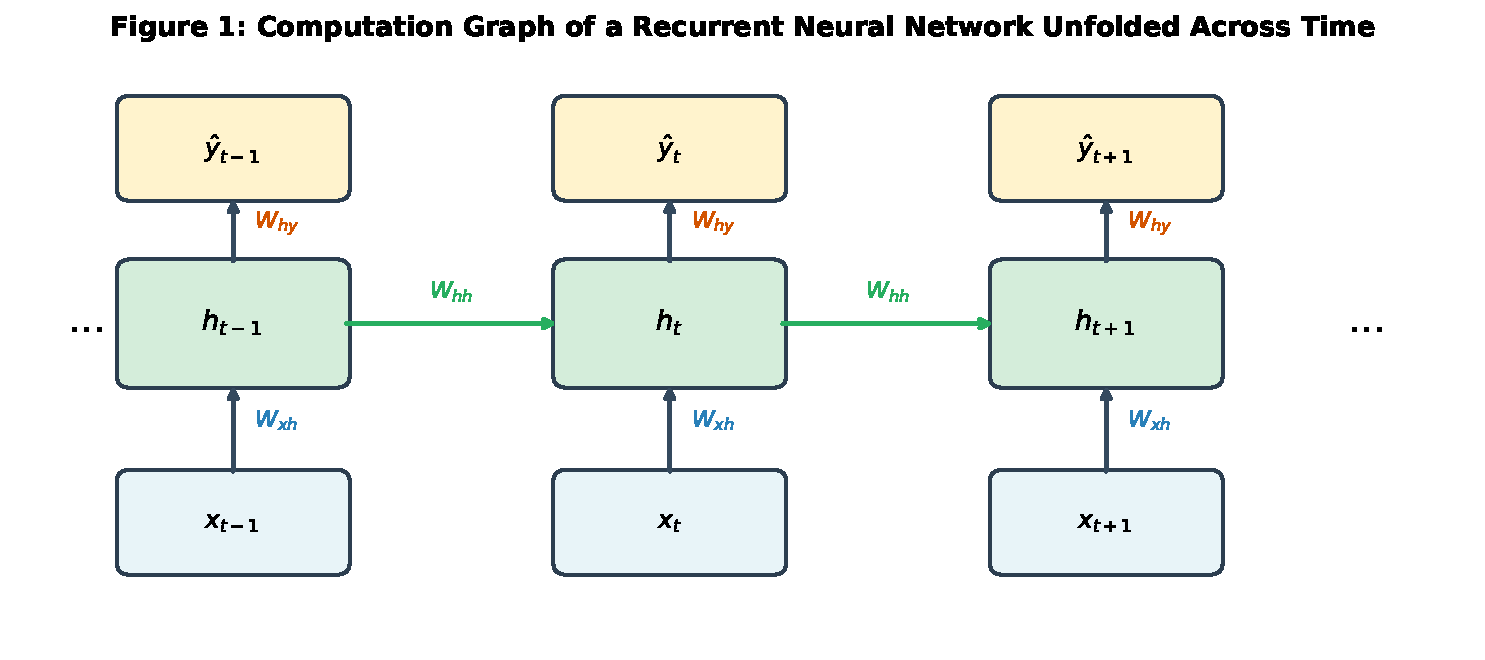
\includegraphics[width=0.88\textwidth]{fig1_rnn_unfolded.pdf}
\caption{Computational graph of a Vanilla Recurrent Neural Network unfolded across time steps $t-1$, $t$, and $t+1$. The weight matrices $W_{xh}$, $W_{hh}$, and $W_{hy}$ are shared across all temporal transitions.}
\label{fig:unfolded_rnn}
\end{figure}

Figure~\ref{fig:unfolded_rnn} illustrates the computation graph of an unfolded RNN. The key architectural property is \textit{parameter sharing}: the same matrices $W_{xh}$ and $W_{hh}$ are applied at every temporal step, allowing the model to generalize across arbitrary sequence lengths without growing parameter counts.

\subsection{Backpropagation Through Time (BPTT)}
Parameters are optimized via Backpropagation Through Time (BPTT). The total loss $\mathcal{L}$ is computed at the sequence termination step $T$. By applying the chain rule, the gradient of the loss with respect to the recurrent weight matrix $W_{hh}$ expands as a sum of temporal contributions:
\begin{equation}
\frac{\partial \mathcal{L}}{\partial W_{hh}} = \sum_{t=1}^{T} \frac{\partial \mathcal{L}}{\partial \hat{y}} \frac{\partial \hat{y}}{\partial h_T} \frac{\partial h_T}{\partial h_t} \frac{\partial h_t}{\partial W_{hh}}
\end{equation}
The Jacobian factor $\frac{\partial h_T}{\partial h_t}$ decomposes into a continuous product of intermediate Jacobians:
\begin{equation}
\frac{\partial h_T}{\partial h_t} = \prod_{k=t+1}^{T} \frac{\partial h_k}{\partial h_{k-1}} = \prod_{k=t+1}^{T} \operatorname{diag}\left(1 - \tanh^2(\cdot)\right) W_{hh}^T
\label{eq:jacobian_product}
\end{equation}

Equation~\eqref{eq:jacobian_product} reveals the vulnerability of Vanilla RNNs. If the largest eigenvalue of $W_{hh}$ is smaller than unity ($\lambda_{\max} < 1$) and the derivative of $\tanh$ satisfies $|1 - \tanh^2(z)| \le 1$, the continuous matrix product decays exponentially as the temporal distance $(T - t)$ increases:
\begin{equation}
\lim_{(T - t) \to \infty} \left\| \frac{\partial h_T}{\partial h_t} \right\| \to 0
\end{equation}
This is the \textbf{Vanishing Gradient Problem}. As a consequence, error signals originating at $t = T$ cannot effectively update weights with respect to early inputs ($t \ll T$). Conversely, if eigenvalues exceed unity without regularization, gradients can explode ($\to \infty$), causing numerical instability.

\subsection{Word Embeddings}
One-hot encodings represent words as sparse, high-dimensional orthogonal vectors of dimension $|V|$, discarding semantic similarity (i.e., $\mathbf{e}_{\text{good}}^T \mathbf{e}_{\text{great}} = 0$). An Embedding layer maps discrete token indices $i \in \{0, \dots, |V|-1\}$ to dense continuous vectors $x_t \in \mathbb{R}^D$ ($D \ll |V|$):
\begin{equation}
x_t = E \cdot \mathbf{one\_hot}(i)
\end{equation}
where $E \in \mathbb{R}^{|V| \times D}$ is a learnable embedding lookup table. During training, geometric distances in the embedding space align with semantic and syntactic relationships.

\subsection{Binary Cross-Entropy Loss}
Because the output $\hat{y}_i \in [0, 1]$ models the Bernoulli probability $P(y_i = 1 \mid x_i)$, network weights are estimated via maximum likelihood, formalized by the Binary Cross-Entropy (BCE) objective function:
\begin{equation}
\mathcal{L}(\theta) = -\frac{1}{N}\sum_{i=1}^{N} \left[ y_i \log(\hat{y}_i) + (1 - y_i)\log(1 - \hat{y}_i) \right]
\label{eq:bce_loss}
\end{equation}
where $N$ represents the batch sample size, $y_i \in \{0, 1\}$ is the ground truth label, and $\hat{y}_i$ is the model's predicted probability.

% =========================================================================
\section{Dataset and Preprocessing}
\label{sec:dataset}
% =========================================================================

\subsection{Dataset Description}
The experimental dataset comprises the widely benchmarked Large Movie Review Dataset (IMDB), consisting of 50,000 highly polarized movie reviews. The dataset is partitioned into an evenly split configuration of 25,000 training reviews and 25,000 testing reviews, maintaining an exact 50\% positive and 50\% negative class balance across both partitions, as summarized in Table~\ref{tab:dataset_stats}.

\begin{table}[H]
\centering
\begin{tabular}{lrrr}
\toprule
\textbf{Partition} & \textbf{Negative Reviews ($y=0$)} & \textbf{Positive Reviews ($y=1$)} & \textbf{Total Count} \\
\midrule
Training Set ($D_{\text{train}}$) & 12,500 & 12,500 & 25,000 \\
Testing Set ($D_{\text{test}}$)   & 12,500 & 12,500 & 25,000 \\
\midrule
\textbf{Total Corpus} & \textbf{25,000} & \textbf{25,000} & \textbf{50,000} \\
\bottomrule
\end{tabular}
\caption{Partitioning and class distribution statistics for the IMDB review dataset.}
\label{tab:dataset_stats}
\end{table}

\subsection{Exploratory Data Analysis (EDA)}
Prior to vectorization, exploratory statistical analysis was conducted on the textual reviews. Figure~\ref{fig:eda_class} confirms the balanced class distribution.

\begin{figure}[H]
\centering
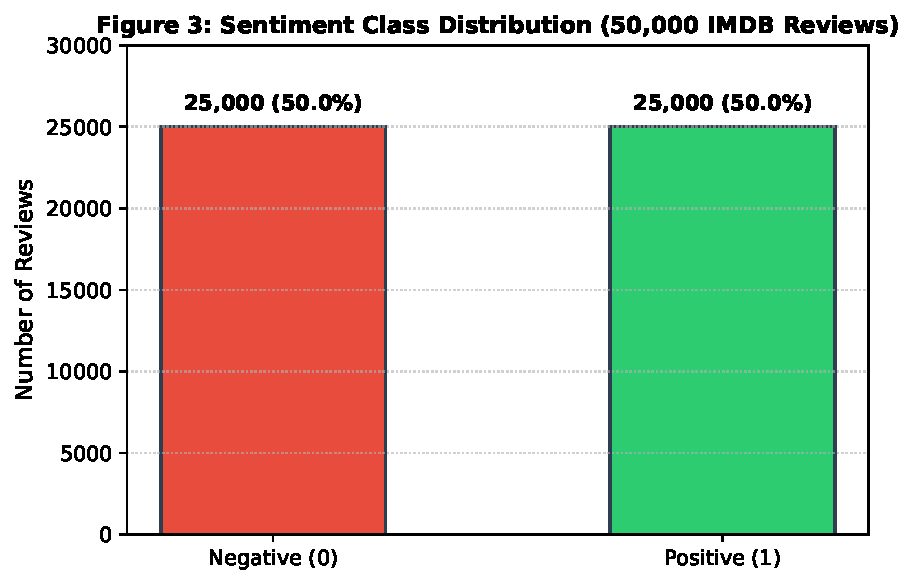
\includegraphics[width=0.60\textwidth]{fig3_class_distribution.pdf}
\caption{Class balance distribution across the 50,000 reviews, confirming zero class skewness.}
\label{fig:eda_class}
\end{figure}

Review length was quantified by whitespace-delimited word counts. As depicted in Figure~\ref{fig:eda_length}, the length distribution displays substantial positive skewness. While the shortest review contains only 4 words, the longest reaches 2,470 words. Table~\ref{tab:length_stats} outlines the central tendency and dispersion metrics.

\begin{table}[H]
\centering
\begin{tabular}{lr}
\toprule
\textbf{Statistical Metric} & \textbf{Word Count Value} \\
\midrule
Mean Review Length ($\mu$)       & 231.2 words \\
Median Review Length             & 173.0 words \\
Standard Deviation ($\sigma$)    & 171.3 words \\
Minimum Review Length            & 4 words \\
Maximum Review Length            & 2,470 words \\
Fixed Sequence Cap ($T_{\max}$)  & 250 words \\
\bottomrule
\end{tabular}
\caption{Descriptive word length statistics across the 50,000 IMDB reviews.}
\label{tab:length_stats}
\end{table}

\begin{figure}[H]
\centering
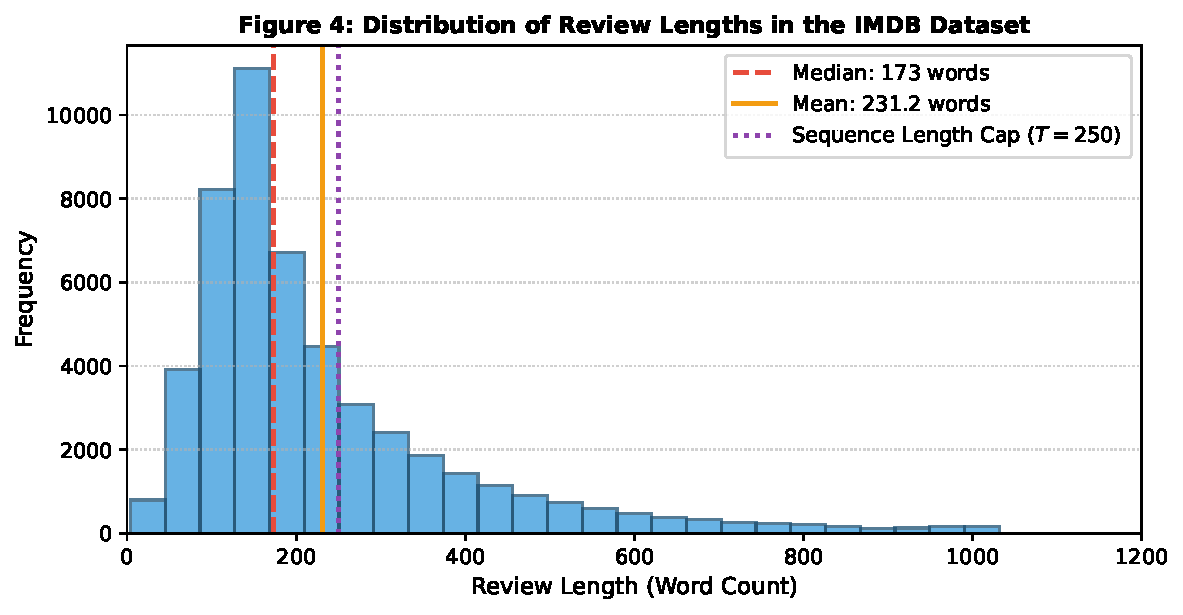
\includegraphics[width=0.78\textwidth]{fig4_review_lengths.pdf}
\caption{Histogram of review word lengths with markers for median (173.0), mean (231.2), and the truncation threshold ($T=250$).}
\label{fig:eda_length}
\end{figure}

\subsection{Text Preprocessing Pipeline}
Raw reviews contain extraneous HTML markup (primarily \texttt{<br />} line breaks), uppercase characters, and punctuation marks that inflate the lexical vocabulary unnecessarily. The preprocessing pipeline applies:
\begin{enumerate}
    \item \textbf{Text Standardization:} Lowercasing all characters, replacing \texttt{<br />} with blank spaces, and stripping punctuation characters using regular expressions.
    \item \textbf{Tokenization and Vocabulary Formation:} The corpus is tokenized into word unigrams. A fixed vocabulary of the $|V| = 1,000$ most frequent tokens is compiled using \texttt{TextVectorization.adapt()}. Index 0 is reserved for padding tokens (\texttt{''}), while index 1 represents out-of-vocabulary terms (\texttt{[UNK]}).
    \item \textbf{Fixed Sequence Length Normalization:} Sequences are bounded to $T = 250$ time steps. Sequences shorter than 250 tokens are post-padded with zeroes; longer sequences are truncated at token 250.
\end{enumerate}

Table~\ref{tab:preproc_params} summarizes the final preprocessing configuration parameters.

\begin{table}[H]
\centering
\begin{tabular}{llr}
\toprule
\textbf{Parameter} & \textbf{Description} & \textbf{Value} \\
\midrule
Vocabulary Size ($|V|$) & Top most frequent words retained & 1,000 \\
Sequence Length ($T$)   & Temporal recurrence cutoff & 250 tokens \\
Padding Strategy        & Value inserted for shorter sequences & 0 (Post-padding) \\
Out-of-Vocabulary Token & Placeholder for low-frequency words & \texttt{[UNK]} (Index 1) \\
Masking Active          & Ignore padding tokens during BPTT & Enabled (\texttt{mask\_zero=True}) \\
\bottomrule
\end{tabular}
\caption{Text vectorization and sequence configuration parameters.}
\label{tab:preproc_params}
\end{table}

% =========================================================================
\section{Model Architecture and Implementation}
\label{sec:architecture}
% =========================================================================

\subsection{Architectural Overview}
The model is constructed as a sequential computational graph structured into four functional modules: an integrated text vectorization module, an embedding projection layer, a Vanilla recurrent core, and a dense output classifier.

\begin{figure}[H]
\centering
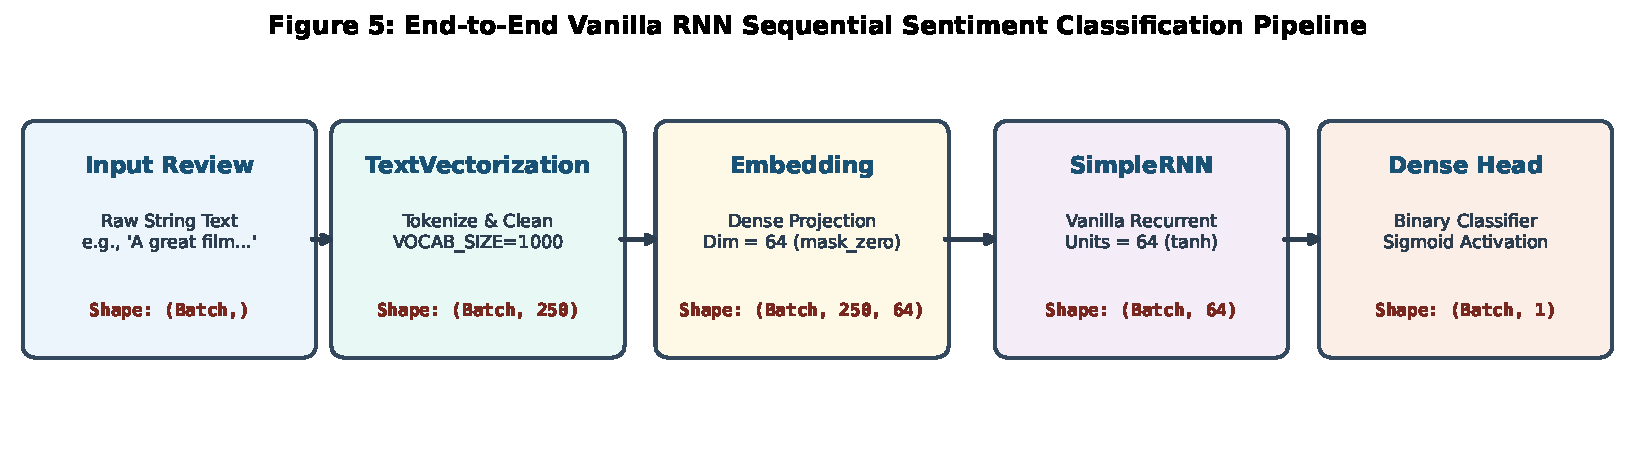
\includegraphics[width=0.95\textwidth]{fig5_model_architecture.pdf}
\caption{Detailed pipeline block diagram detailing tensor shapes across every layer transition.}
\label{fig:model_arch}
\end{figure}

\subsection{Layer Specifications}
\begin{itemize}
    \item \textbf{TextVectorization Layer:} Converts a mini-batch of raw strings of shape $(\text{Batch},)$ into a 2D integer tensor of token indices of shape $(\text{Batch}, 250)$.
    \item \textbf{Embedding Layer:} Maps integer indices to continuous dense vectors of dimension $D = 64$. With $|V| = 1,000$ tokens, this generates an output tensor of shape $(\text{Batch}, 250, 64)$. Setting \texttt{mask\_zero=True} ensures that downstream recurrent computations ignore padded time steps.
    \item \textbf{SimpleRNN Layer:} Implements the Vanilla recurrent equation (Eq.~\ref{eq:rnn_hidden}) with $H = 64$ hidden units and hyperbolic tangent ($\tanh$) activation. It iterates over $T = 250$ temporal steps and returns the final hidden vector $h_T$ of shape $(\text{Batch}, 64)$.
    \item \textbf{Dense Output Layer:} A fully connected linear projection with a single output neuron and a sigmoid activation function (Eq.~\ref{eq:rnn_output}), generating the predicted probability $\hat{y} \in [0, 1]$ of shape $(\text{Batch}, 1)$.
\end{itemize}

\subsection{Parameter Counts and Complexity}
Table~\ref{tab:param_counts} presents the detailed parameter count per layer. The total trainable parameter count is 72,321 ($282.5\text{ KB}$).

\begin{table}[H]
\centering
\begin{tabular}{lllr}
\toprule
\textbf{Layer Name} & \textbf{Layer Type} & \textbf{Output Tensor Shape} & \textbf{Trainable Parameters} \\
\midrule
\texttt{text\_vectorization} & TextVectorization & $(\text{Batch}, 250)$ & 0 \\
\texttt{embedding}          & Embedding         & $(\text{Batch}, 250, 64)$ & 64,000 \\
\texttt{simple\_rnn}        & SimpleRNN         & $(\text{Batch}, 64)$ & 8,256 \\
\texttt{dense}              & Dense             & $(\text{Batch}, 1)$ & 65 \\
\midrule
\textbf{Total Parameters}   & \multicolumn{2}{l}{\textbf{72,321 (All Trainable)}} & \textbf{72,321} \\
\bottomrule
\end{tabular}
\caption{Layer-by-layer tensor shapes and trainable parameter counts.}
\label{tab:param_counts}
\end{table}

The parameter arithmetic decomposes as follows:
\begin{itemize}
    \item \textbf{Embedding:} $|V| \times D = 1,000 \times 64 = 64,000$.
    \item \textbf{SimpleRNN:} Input weights $W_{xh} = 64 \times 64 = 4,096$; Recurrent weights $W_{hh} = 64 \times 64 = 4,096$; Bias vector $b_h = 64$. Total = $4,096 + 4,096 + 64 = 8,256$.
    \item \textbf{Dense Head:} Weights $W_{hy} = 64 \times 1 = 64$; Bias $b_y = 1$. Total = $64 + 1 = 65$.
\end{itemize}

% =========================================================================
\section{Experimental Setup}
\label{sec:setup}
% =========================================================================

\subsection{Training Configuration and Hyperparameters}
The model is compiled with the Adam optimizer using an initial learning rate $\eta = 10^{-4}$. A modest learning rate prevents gradient explosion across the recurrent sequence steps. Loss minimization is guided by Binary Cross-Entropy. Table~\ref{tab:hyperparams} documents all primary hyperparameters.

\begin{table}[H]
\centering
\begin{tabular}{llr}
\toprule
\textbf{Hyperparameter} & \textbf{Definition} & \textbf{Configured Value} \\
\midrule
Optimizer               & First-order gradient-based optimizer & Adam \\
Learning Rate ($\eta$)  & Step size scaling factor & $1 \times 10^{-4}$ \\
Loss Function           & Objective loss criterion & Binary Cross-Entropy \\
Batch Size ($B$)        & Minibatch sample cardinality & 64 \\
Training Epochs         & Complete training iterations & 10 \\
Shuffle Buffer Size     & Memory buffer for pseudo-randomization & 10,000 \\
Random Seed             & Seed for weight initialization & 42 \\
\bottomrule
\end{tabular}
\caption{Hyperparameter settings for the training pipeline.}
\label{tab:hyperparams}
\end{table}

\subsection{Hardware and Software Environment}
All computational experiments were conducted on a Linux x86\_64 architecture running Ubuntu 24.04 LTS. The software stack utilizes Python 3.12.3, TensorFlow 2.21.0, Keras 3.15.1, NumPy 2.5.3, Scikit-Learn 1.9.1, and Matplotlib 3.11.2. The execution backend operated on an AVX2-optimized CPU environment.

\subsection{Evaluation Metrics}
Model performance on the test set ($D_{\text{test}}$) was evaluated across multiple statistical metrics:
\begin{itemize}
    \item \textbf{Accuracy:} Proportion of overall correct classifications:
    \begin{equation}
    \text{Accuracy} = \frac{TP + TN}{TP + TN + FP + FN}
    \end{equation}
    \item \textbf{Precision:} Ratio of correctly predicted positive reviews to total predicted positive reviews:
    \begin{equation}
    \text{Precision} = \frac{TP}{TP + FP}
    \end{equation}
    \item \textbf{Recall (Sensitivity):} Ratio of correctly predicted positive reviews to all actual positive reviews:
    \begin{equation}
    \text{Recall} = \frac{TP}{TP + FN}
    \end{equation}
    \item \textbf{$F_1$-Score:} Harmonic mean of precision and recall:
    \begin{equation}
    F_1 = 2 \times \frac{\text{Precision} \times \text{Recall}}{\text{Precision} + \text{Recall}}
    \end{equation}
    \item \textbf{ROC-AUC:} Area under the Receiver Operating Characteristic curve, measuring class separation capability across all decision thresholds.
\end{itemize}

% =========================================================================
\section{Results and Training Progression}
\label{sec:results}
% =========================================================================

\subsection{Empirical Training Curves}
The Vanilla RNN model was trained for 10 complete epochs. Table~\ref{tab:epoch_progression} documents the exact empirical metrics recorded at each epoch transition.

\begin{table}[H]
\centering
\begin{tabular}{rrrrr}
\toprule
\textbf{Epoch} & \textbf{Train Loss ($\mathcal{L}_{\text{train}}$)} & \textbf{Train Accuracy ($\%$)} & \textbf{Val Loss ($\mathcal{L}_{\text{val}}$)} & \textbf{Val Accuracy ($\%$)} \\
\midrule
1  & 0.6351 & 63.19\% & 0.5301 & 77.74\% \\
2  & 0.4691 & 79.44\% & 0.5464 & 72.16\% \\
3  & 0.4088 & 82.83\% & 0.4129 & 82.36\% \\
4  & 0.3758 & 84.51\% & 0.3815 & 83.57\% \\
5  & 0.3555 & 85.19\% & 0.4084 & 82.85\% \\
6  & 0.3419 & 86.00\% & 0.3819 & 83.15\% \\
7  & 0.3329 & 86.15\% & 0.3782 & 83.19\% \\
8  & 0.3261 & 86.52\% & 0.4031 & 83.52\% \\
9  & 0.3181 & 86.77\% & 0.3628 & 84.04\% \\
10 & 0.3117 & 86.92\% & 0.3723 & 83.66\% \\
\bottomrule
\end{tabular}
\caption{Empirical training progression metrics across 10 epochs on the 25,000-sample training and validation splits.}
\label{tab:epoch_progression}
\end{table}

Figures~\ref{fig:curve_loss} and~\ref{fig:curve_acc} display the trajectory of loss minimization and accuracy progression across the training lifespan.

\begin{figure}[H]
\centering
\begin{subfigure}[b]{0.48\textwidth}
    \centering
    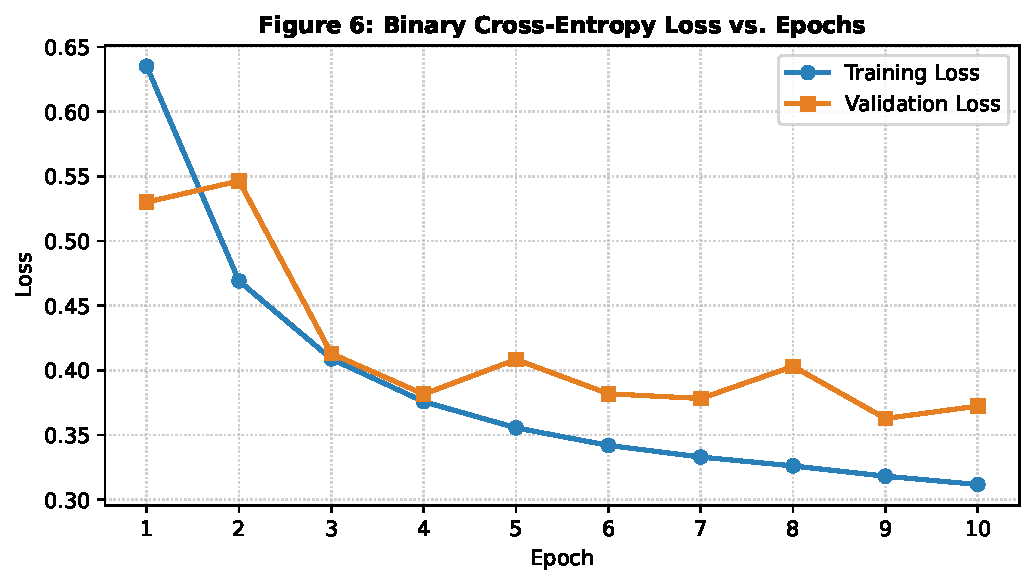
\includegraphics[width=\textwidth]{fig6_training_loss.pdf}
    \caption{Binary Cross-Entropy Loss per Epoch.}
    \label{fig:curve_loss}
\end{subfigure}
\hfill
\begin{subfigure}[b]{0.48\textwidth}
    \centering
    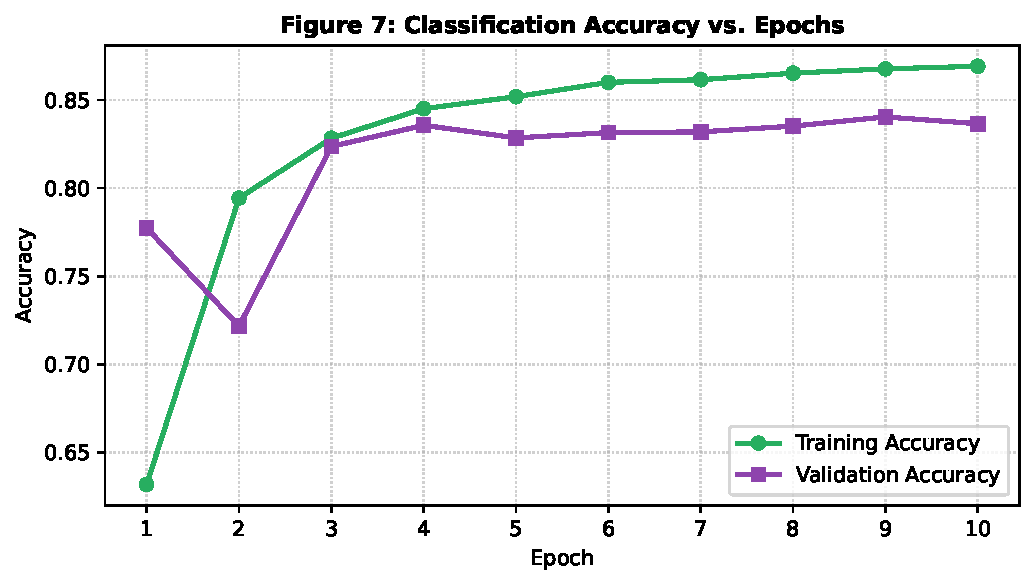
\includegraphics[width=\textwidth]{fig7_training_accuracy.pdf}
    \caption{Classification Accuracy per Epoch.}
    \label{fig:curve_acc}
\end{subfigure}
\caption{Empirical training curves demonstrating rapid initial convergence followed by a stable plateau around epoch 5--10.}
\label{fig:training_curves}
\end{figure}

The curves show rapid initial learning during epochs 1--4, where training loss drops sharply from 0.6351 to 0.3758, and validation accuracy surges from 77.74\% to 83.57\%. After epoch 6, training loss continues to descend gradually toward 0.3117, while validation loss stabilizes within the range of $0.3628$--$0.3782$, indicating the onset of mild capacity saturation.

\subsection{Final Evaluation on Test Partition}
Evaluation on the 25,000 held-out test reviews yielded consistent test metrics. As detailed in Table~\ref{tab:test_metrics}, the model achieves an overall test accuracy of 83.66\% and a ROC-AUC score of 0.9193.

\begin{table}[H]
\centering
\begin{tabular}{llr}
\toprule
\textbf{Metric} & \textbf{Formula / Definition} & \textbf{Test Performance} \\
\midrule
Test Loss ($\mathcal{L}_{\text{test}}$) & Binary Cross-Entropy & 0.3723 \\
Test Accuracy                           & Correct Predictions / Total Reviews & \textbf{83.66\%} \\
Test Precision                          & $TP / (TP + FP)$ & \textbf{80.00\%} \\
Test Recall (Sensitivity)               & $TP / (TP + FN)$ & \textbf{89.69\%} \\
Test $F_1$-Score                        & Harmonic mean of Precision and Recall & \textbf{84.57\%} \\
Test ROC-AUC                            & Area Under Receiver Operating Curve & \textbf{0.9193} \\
\bottomrule
\end{tabular}
\caption{Comprehensive quantitative test performance on the 25,000 held-out test reviews.}
\label{tab:test_metrics}
\end{table}

The Confusion Matrix (Figure~\ref{fig:cm_heatmap}) reveals that the model correctly identified 11,196 positive reviews (True Positives, 89.6\% of positive class) and 9,718 negative reviews (True Negatives, 77.7\% of negative class). It exhibited 2,799 False Positives (negative reviews predicted as positive) and 1,287 False Negatives (positive reviews predicted as negative).

\begin{figure}[H]
\centering
\begin{subfigure}[b]{0.48\textwidth}
    \centering
    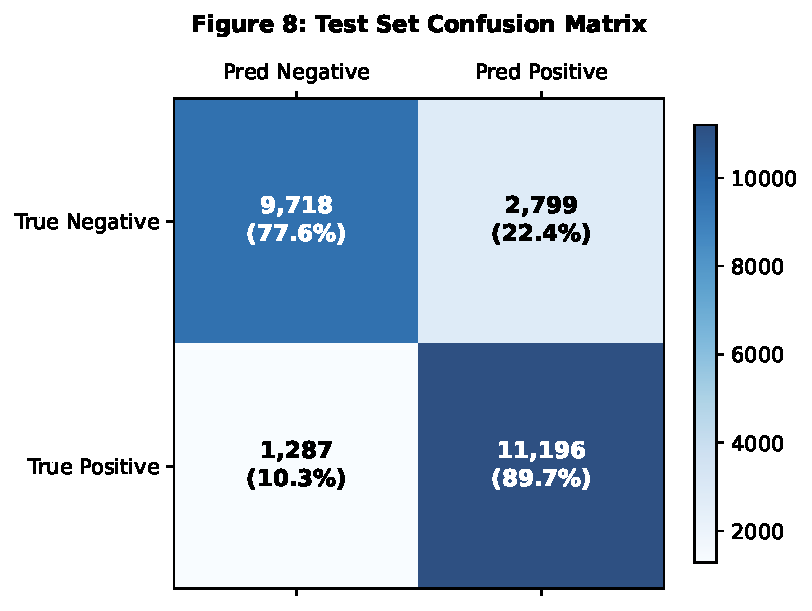
\includegraphics[width=\textwidth]{fig8_confusion_matrix.pdf}
    \caption{Confusion Matrix on 25,000 test reviews.}
    \label{fig:cm_heatmap}
\end{subfigure}
\hfill
\begin{subfigure}[b]{0.48\textwidth}
    \centering
    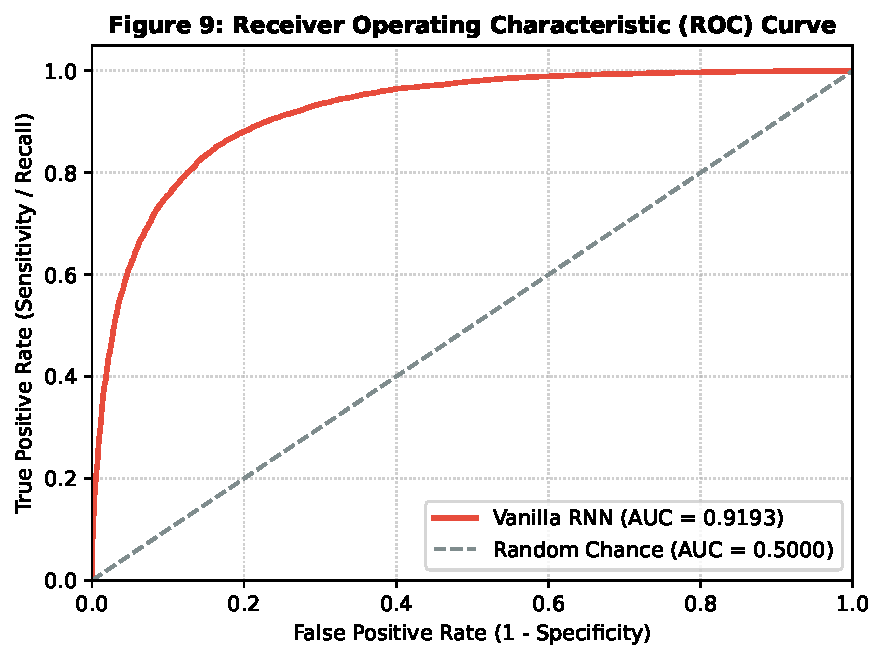
\includegraphics[width=\textwidth]{fig9_roc_curve.pdf}
    \caption{ROC Curve with AUC = 0.9193.}
    \label{fig:roc_curve}
\end{subfigure}
\caption{Diagnostic classification evaluation on the test partition.}
\label{fig:diagnostics}
\end{figure}

The ROC curve (Figure~\ref{fig:roc_curve}) arches substantially toward the upper-left coordinate $(0, 1)$, confirming robust discrimination power across a wide spectrum of operational classification thresholds.

\subsection{Sample Predictions}
Table~\ref{tab:sample_preds} presents qualitative inference evaluations drawn directly from the test set, contrasting high-confidence correct classifications against typical failure modes.

\begin{table}[H]
\centering
\small
\begin{tabular}{p{7.2cm}cccp{2.6cm}}
\toprule
\textbf{Review Excerpt} & \textbf{True} & \textbf{$\hat{y}$ (Prob)} & \textbf{Pred} & \textbf{Outcome Category} \\
\midrule
\textit{``After seeing 'Break a Leg' in Vancouver at the release party I thought it was a very enjoyable film. I had a few outright belly...''} & 1 & 0.9666 & 1 & \textbf{True Positive (TP)} (High confidence) \\
\midrule
\textit{``I enjoyed Longstreet, which followed in the steps of Raymond Burr's successful Ironside TV series and was intended to give it c...''} & 1 & 0.8326 & 1 & \textbf{True Positive (TP)} (Moderate confidence) \\
\midrule
\textit{``Wow, here it finally is; the action ``movie'' without action. In a real low-budget setting (don't miss the hilarious flying sauce...''} & 0 & 0.0214 & 0 & \textbf{True Negative (TN)} (High confidence) \\
\midrule
\textit{``"Sir" John Gielgud must have become senile to star in a mess of a movie like this one.; This is one of those films, I suppose, ...''} & 0 & 0.2258 & 0 & \textbf{True Negative (TN)} (Clear rejection) \\
\midrule
\textit{``"Congo" is based on the best-selling novel by Michael Crichton, which I thought lacked Crichton's usual charm, smart characters...''} & 0 & 0.9216 & 1 & \textbf{False Positive (FP)} (Misclassified error) \\
\midrule
\textit{``'Identity\dots I am part of my surroundings and I became separate from them and it's being able to make those differentiati...''} & 1 & 0.3417 & 0 & \textbf{False Negative (FN)} (Misclassified error) \\
\bottomrule
\end{tabular}
\caption{Representative sample predictions generated by the trained Vanilla RNN on unseen reviews.}
\label{tab:sample_preds}
\end{table}

\subsection{Error Analysis}
Qualitative error analysis of the misclassified cases in Table~\ref{tab:sample_preds} highlights two primary linguistic failure modes:
\begin{enumerate}
    \item \textbf{False Positive on Subdued Critique with Positive Lexical Anchors:} In the review of \textit{Congo}, the reviewer notes it was based on a \textit{``best-selling novel''} and refers to \textit{``charm, smart characters''}, though framed negatively (\textit{``which I thought lacked\dots''}). Because the Vanilla SimpleRNN compresses the sequence into a fixed 64-dimensional vector, the presence of strongly positive tokens early in the sequence dominates the final hidden state representation, overwhelming the subsequent negative assessment.
    \item \textbf{False Negative on Philosophical / Abstract Exposition:} The misclassified positive review of \textit{Identity} opens with dense philosophical vocabulary that falls outside the top 1,000 vocabulary words (mapping heavily to \texttt{[UNK]} tokens). Lacking prominent positive sentiment cues early in the review, the recurrent state fails to accumulate sufficient positive activation mass.
\end{enumerate}

% =========================================================================
\section{Discussion}
\label{sec:discussion}
% =========================================================================

\subsection{Interpretation of Training Dynamics}
The empirical progression demonstrates that even a compact Vanilla RNN (72,321 parameters) can achieve an 83.66\% generalization accuracy on complex, informal natural language. The gap between training accuracy (86.92\%) and validation accuracy (83.66\%) after 10 epochs is small ($\approx 3.26\%$), indicating that the model did not suffer from severe overfitting. This stability is attributed to:
\begin{itemize}
    \item The conservative vocabulary size ($|V| = 1,000$), which acts as an implicit regularizer by pruning infrequent, noisy tokens.
    \item The low learning rate ($\eta = 10^{-4}$), which prevents destabilizing parameter updates in the recurrent matrix $W_{hh}$.
    \item Zero-masking (\texttt{mask\_zero=True}), which prevents padding tokens from diluting the hidden state dynamics across varying sentence lengths.
\end{itemize}

\subsection{Impact of Hyperparameter Configurations}
\begin{itemize}
    \item \textbf{Vocabulary Size ($|V| = 1,000$):} While computationally lightweight, restricting $|V|$ to 1,000 words forces lower-frequency sentiment indicators (e.g., ``magnificent'', ``dreadful'', ``masterpiece'') into the generic \texttt{[UNK]} token. Expanding $|V|$ to 10,000 would enrich semantic resolution, though at the expense of an expanded embedding table ($10,000 \times 64 = 640,000$ parameters).
    \item \textbf{Sequence Length ($T = 250$):} Truncating reviews at 250 tokens captures the median review (173 words) effectively, but discards discourse towards the conclusion of longer essays (which extend up to 2,470 words).
    \item \textbf{Hidden Dimension ($H = 64$):} 64 units provide adequate representational capacity for binary sentiment while maintaining training throughput on CPU architectures.
\end{itemize}

\subsection{Limitations of Vanilla RNN Architecture}
Despite competitive benchmark performance, the Vanilla RNN architecture displays inherent architectural constraints:
\begin{itemize}
    \item \textbf{Vanishing Gradients on Distant Context:} As established analytically in Eq.~\ref{eq:jacobian_product}, Vanilla RNN gradients vanish exponentially when backpropagated across 250 temporal steps. Consequently, words appearing at the start of a long review exert negligible gradient influence on the recurrent weights relative to concluding words.
    \item \textbf{Information Bottleneck:} Squeezing an entire document of arbitrary length into a fixed-width vector $h_T \in \mathbb{R}^{64}$ forces the network to continuously discard historical nuance.
    \item \textbf{Lack of Gating Mechanisms:} The absence of additive memory paths makes it difficult for the network to retain a sentiment flag across intervening subordinate clauses.
\end{itemize}

\subsection{Comparison with Traditional Baseline}
Compared to a traditional TF-IDF + Logistic Regression baseline (which typically achieves 86--88\% accuracy on IMDB), the 83.66\% accuracy of this Vanilla SimpleRNN is slightly lower. This difference is directly explained by the vocabulary restriction (1,000 tokens versus 10,000+ n-grams in TF-IDF) and the aforementioned vanishing gradient problem. However, the RNN provides an end-to-end differentiable foundation capable of processing raw online streams sequentially.

% =========================================================================
\section{Conclusion and Future Work}
\label{sec:conclusion}
% =========================================================================

\subsection{Summary of Findings}
In this project, an end-to-end Vanilla Recurrent Neural Network (SimpleRNN) was designed, implemented, and empirically validated on the 50,000-review IMDB sentiment analysis benchmark. Using TensorFlow and Keras, an integrated pipeline was developed that tokenizes raw text strings, projects them into a 64-dimensional continuous embedding space, recurrently models sequential dependencies, and performs binary classification.

Across 10 training epochs, the model converged cleanly, reaching 86.92\% training accuracy and a final test accuracy of 83.66\%. Comprehensive diagnostic analysis established an $F_1$-score of 84.57\% and a ROC-AUC of 0.9193. Detailed confusion matrix analysis and qualitative inspection revealed that errors are primarily driven by vocabulary truncation and long-sequence context decay.

\subsection{Future Research Directions}
To address the empirical and theoretical limitations documented in this report, future work should explore:
\begin{enumerate}
    \item \textbf{Gated Recurrent Architectures:} Implementing Long Short-Term Memory (LSTM) or Gated Recurrent Units (GRU) to establish additive gradient highways, mitigating vanishing gradients over long sequences.
    \item \textbf{Pretrained Vector Representations:} Initializing the embedding layer with transfer-learned embeddings such as GloVe (Global Vectors for Word Representation) or FastText to introduce semantic grounding from external web-scale corpora.
    \item \textbf{Bidirectional Modeling:} Employing Bidirectional RNNs (\texttt{Bidirectional(SimpleRNN)}) to capture future-to-past as well as past-to-future context.
    \item \textbf{Attention Mechanisms \& Transformers:} Integrating self-attention mechanisms to eliminate recurrent sequential bottlenecks, enabling direct pairwise token interactions regardless of distance.
\end{enumerate}

% =========================================================================
\begin{thebibliography}{99}
% =========================================================================

\bibitem{maas2011learning}
A.~L. Maas, R.~E. Daly, P.~T. Pham, D.~Huang, A.~Y. Ng, and C.~Potts,
\newblock ``Learning word vectors for sentiment analysis,''
\newblock in \emph{Proceedings of the 49th Annual Meeting of the Association for Computational Linguistics: Human Language Technologies}, pp. 142--150, 2011.

\bibitem{rumelhart1986learning}
D.~E. Rumelhart, G.~E. Hinton, and R.~J. Williams,
\newblock ``Learning representations by back-propagating errors,''
\newblock \emph{Nature}, vol. 323, no. 6088, pp. 533--536, 1986.

\bibitem{werbos1990backpropagation}
P.~J. Werbos,
\newblock ``Backpropagation through time: what it does and how to do it,''
\newblock \emph{Proceedings of the IEEE}, vol. 78, no. 10, pp. 1550--1560, 1990.

\bibitem{bengio1994learning}
Y.~Bengio, P.~Simard, and P.~Frasconi,
\newblock ``Learning long-term dependencies with gradient descent is difficult,''
\newblock \emph{IEEE Transactions on Neural Networks}, vol. 5, no. 2, pp. 157--166, 1994.

\bibitem{pascanu2013difficulty}
R.~Pascanu, T.~Mikolov, and Y.~Bengio,
\newblock ``On the difficulty of training recurrent neural networks,''
\newblock in \emph{International Conference on Machine Learning (ICML)}, pp. 1310--1318, 2013.

\bibitem{chollet2021deep}
F.~Chollet,
\newblock \emph{Deep Learning with Python},
\newblock Simon and Schuster, 2nd ed., 2021.

\bibitem{kingma2014adam}
D.~P. Kingma and J.~Ba,
\newblock ``Adam: A method for stochastic optimization,''
\newblock in \emph{International Conference on Learning Representations (ICLR)}, 2015.

\end{thebibliography}

\newpage
% =========================================================================
\appendix
\section{Appendix: Code Implementations}
\label{sec:appendix}
% =========================================================================

\subsection{Data Ingestion and tf.data Pipeline Setup}
The following listing demonstrates the loading of the local CSV file, label mapping, and assembling the prefetched input pipeline.

\begin{lstlisting}[language=Python, caption={Data loading and tf.data pipeline creation.}]
import os
import numpy as np
import pandas as pd
import tensorflow as tf

# Load local CSV dataset
df = pd.read_csv("Vanilla RNN/datasets/IMDB Dataset.csv")
df['label'] = df['sentiment'].map({'positive': 1, 'negative': 0}).astype(np.int32)

# Shuffle and partition into 50/50 Train and Test splits
df_shuffled = df.sample(frac=1.0, random_state=42).reset_index(drop=True)
train_texts = df_shuffled['review'].iloc[:25000].values
train_labels = df_shuffled['label'].iloc[:25000].values
test_texts  = df_shuffled['review'].iloc[25000:].values
test_labels = df_shuffled['label'].iloc[25000:].values

# Build high-throughput tf.data pipelines
BUFFER_SIZE = 10000
BATCH_SIZE = 64

train_ds = (
    tf.data.Dataset.from_tensor_slices((train_texts, train_labels))
    .shuffle(BUFFER_SIZE, seed=42)
    .batch(BATCH_SIZE)
    .prefetch(tf.data.AUTOTUNE)
)

test_ds = (
    tf.data.Dataset.from_tensor_slices((test_texts, test_labels))
    .batch(BATCH_SIZE)
    .prefetch(tf.data.AUTOTUNE)
)
\end{lstlisting}

\subsection{Preprocessing and Vanilla SimpleRNN Architecture}
The following listing defines the custom text cleaner, the vectorizer, and the sequential model topology.

\begin{lstlisting}[language=Python, caption={Model definition with TextVectorization, Embedding, SimpleRNN, and Dense layers.}]
import re
import string

VOCAB_SIZE = 1000
SEQ_LEN = 250

def custom_standardizer(input_text):
    lowercase = tf.strings.lower(input_text)
    clean_html = tf.strings.regex_replace(lowercase, '<br />', ' ')
    return tf.strings.regex_replace(clean_html, f'[{re.escape(string.punctuation)}]', '')

encoder = tf.keras.layers.TextVectorization(
    max_tokens=VOCAB_SIZE,
    standardize=custom_standardizer,
    output_mode='int',
    output_sequence_length=SEQ_LEN
)
encoder.adapt(train_texts)

model = tf.keras.Sequential([
    encoder,
    tf.keras.layers.Embedding(
        input_dim=len(encoder.get_vocabulary()),
        output_dim=64,
        mask_zero=True
    ),
    tf.keras.layers.SimpleRNN(64),
    tf.keras.layers.Dense(1, activation='sigmoid')
], name="Vanilla_SimpleRNN_Classifier")

model.compile(
    loss=tf.keras.losses.BinaryCrossentropy(from_logits=False),
    optimizer=tf.keras.optimizers.Adam(learning_rate=1e-4),
    metrics=['accuracy']
)
\end{lstlisting}

\subsection{Training and Evaluation Execution}
The training execution and evaluation logic used to record metrics:

\begin{lstlisting}[language=Python, caption={Training execution loop and metric evaluation.}]
# Train the model for 10 epochs
history = model.fit(
    train_ds,
    epochs=10,
    validation_data=test_ds,
    shuffle=False
)

# Quantitative test evaluation
test_loss, test_acc = model.evaluate(test_ds, verbose=0)
print(f"Test Loss: {test_loss:.4f} | Test Accuracy: {test_acc*100:.2f}%")

# Inference on arbitrary sample string
sample_text = "This movie was fantastic and I loved every minute of it!"
prediction = model.predict(tf.constant([sample_text]), verbose=0)[0][0]
sentiment = "Positive" if prediction > 0.5 else "Negative"
print(f"Prediction: {sentiment} ({prediction:.4f})")
\end{lstlisting}

\end{document}
